% !TeX spellcheck = de_DE
\section{\ExercisePrefixEmbeddedC Android Bluetooth Low Energy \optional}
\newcommand{\toolAble}{\textsc{ABLE}\xspace}
\toolAble (Android Bluetooth Low Energy) ist eine Applikation für Androidgeräte, um über BLE (Bluetooth Low Energy) eine drahtlose Verbindung zwischen einem Android-Smartphone und einem anderen BLE-Gerät herzustellen.
Der Mikrocontroller des C/C++-Praktikums kann durch ein zusätzliches Modul mit BLE erweitert werden.
Du kannst auf einem Androidgerät die \toolAble-App installieren und dich mit dem Mikrocontroller verbinden.
\Cref{fig:ablePreview} zeigt ein Beispielprogramm, in dem der Mikrocontroller den X-Wert des Joysticks~1 über BLE an ein Android-Smartphone sendet.
Eine ausführliche Anleitung zur Nutzung von \toolAble auf dem Mikrocontroller des Praktikums findest du unter \href{https://github.com/Echtzeitsysteme/able/wiki/Cpp-Lab-Tutorial}{diesem Link [1]}. 
\begin{figure}[!htb]
	\centering
	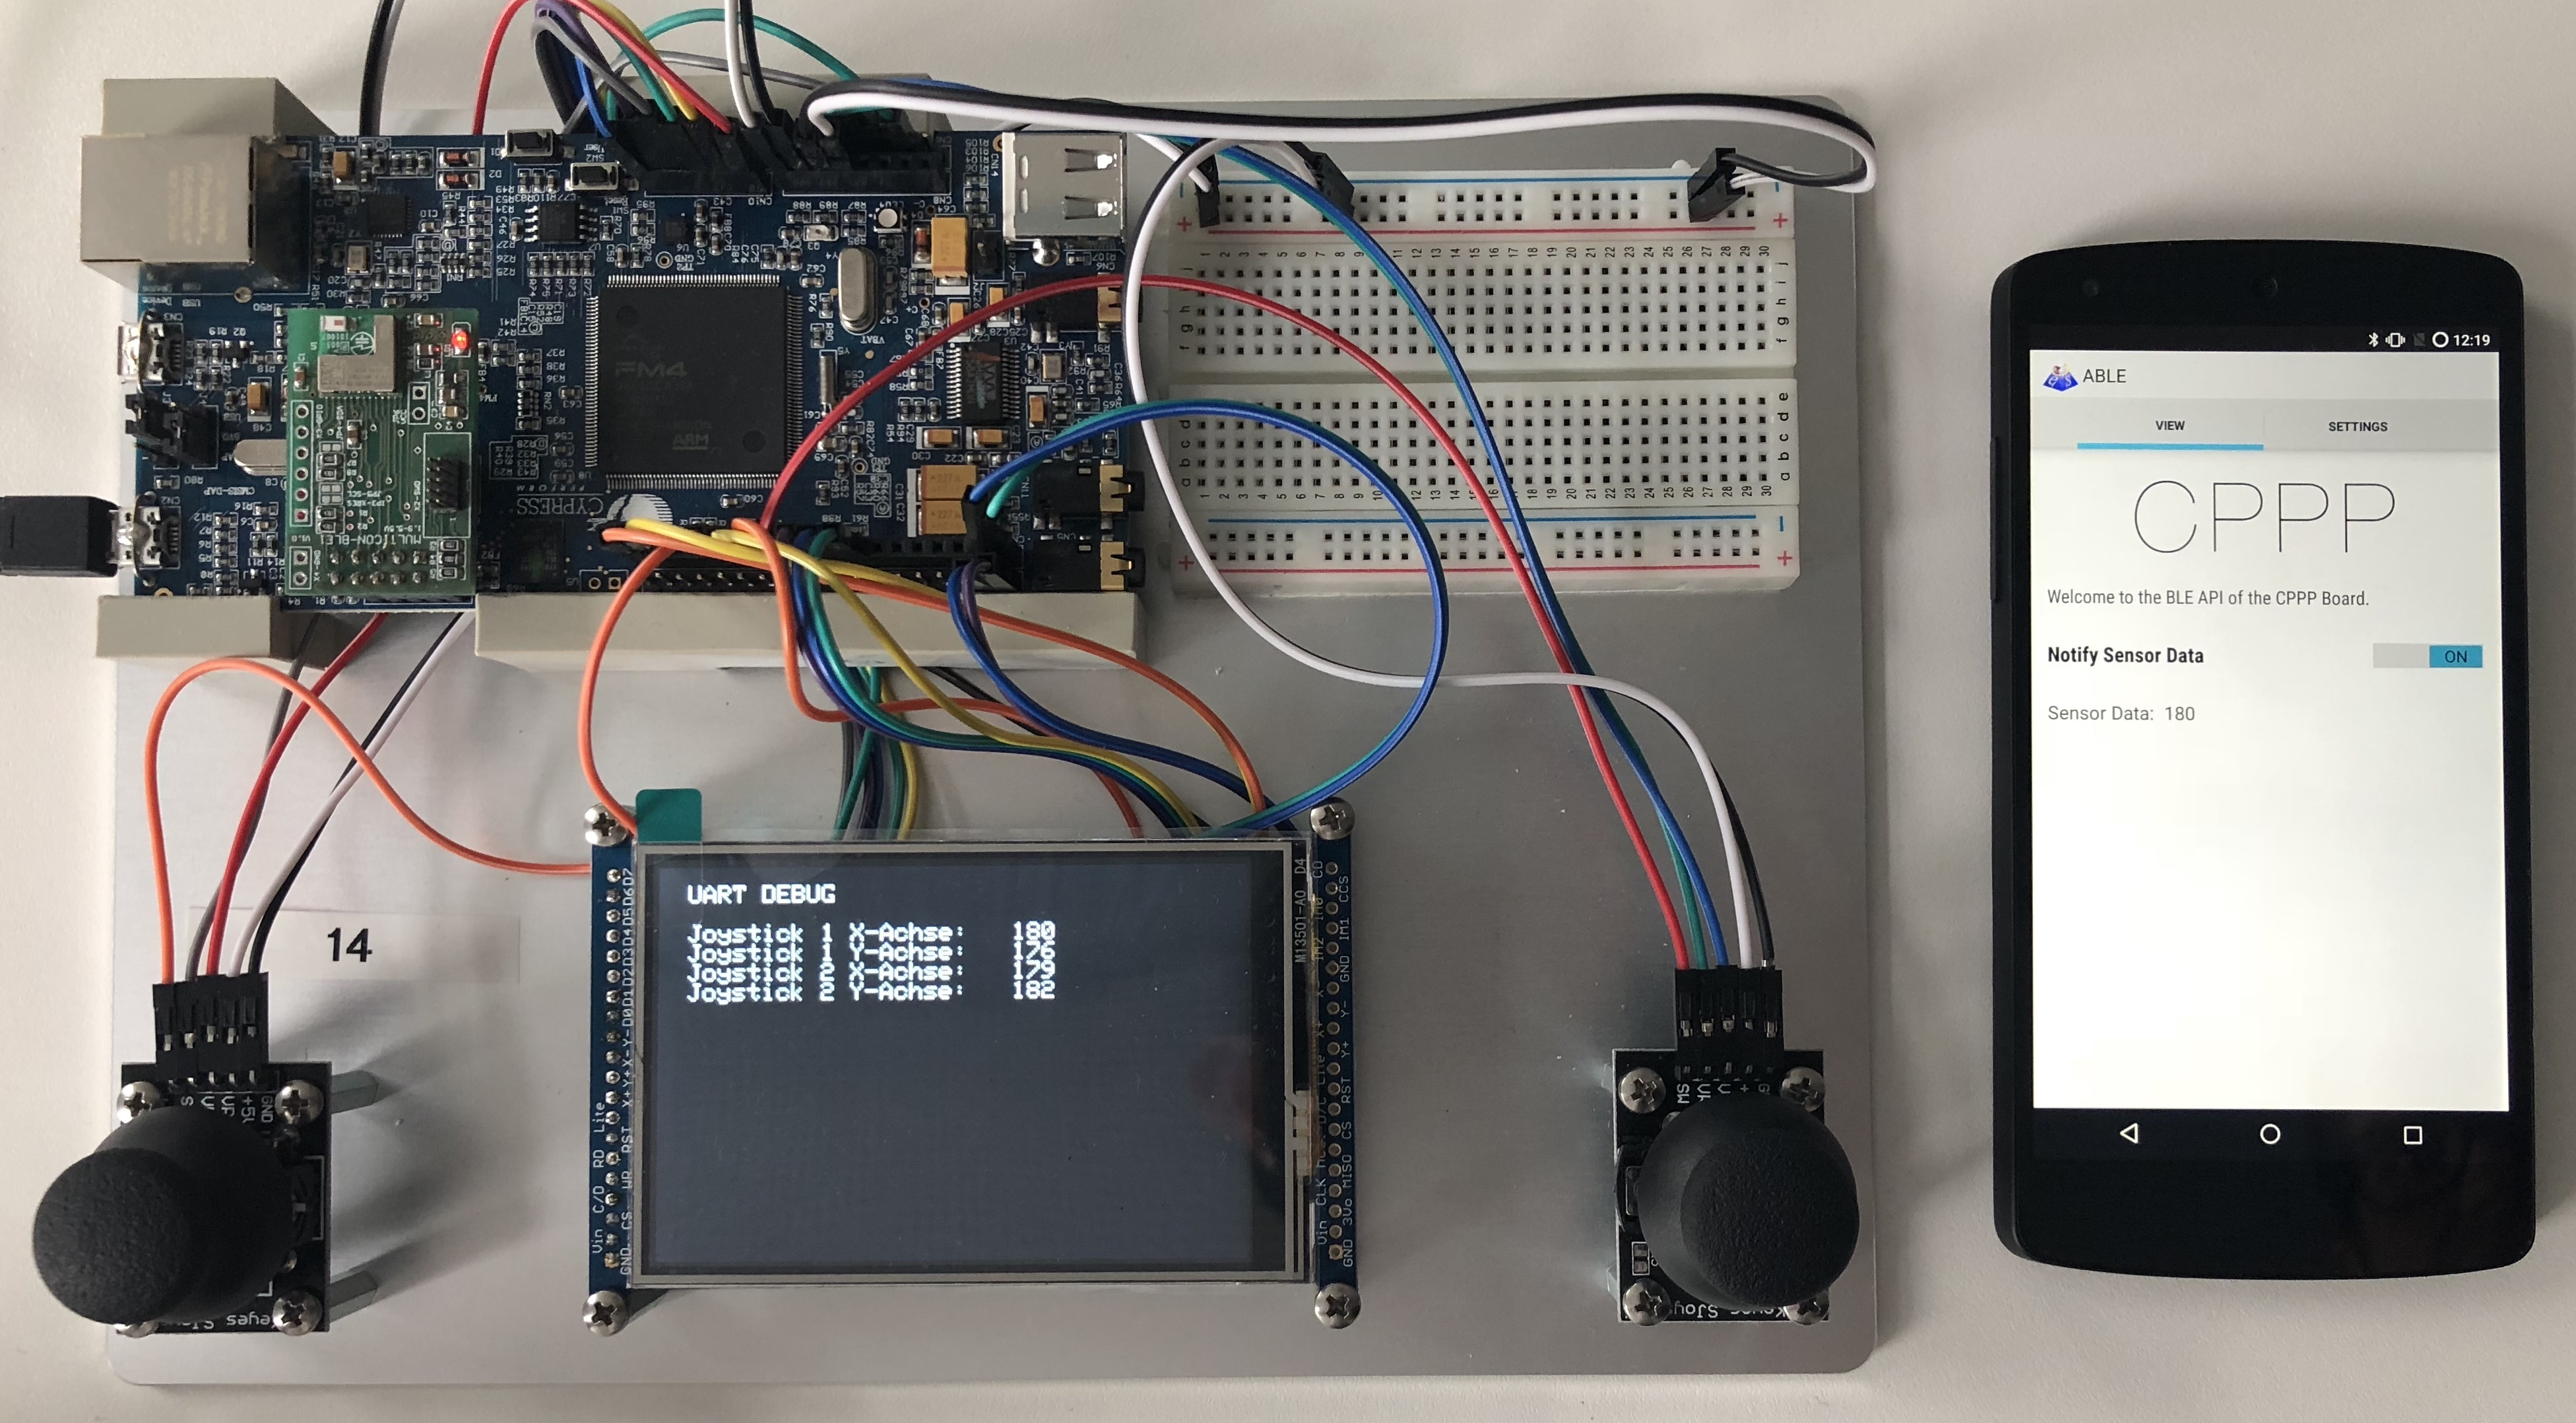
\includegraphics[width=0.9\textwidth]{./05_c/figures/ABLE_preview.jpg}
	\caption{\toolAble: Der Microcontroller verbunden über Bluetooth mit einem Androidgeräte}
	\label{fig:ablePreview}
\end{figure} 
